\documentclass[a4paper,10pt]{article}
\usepackage[utf8]{inputenc}
\usepackage{amstext}
\usepackage{listings}
\usepackage{graphicx}
\usepackage{subfigure}
\usepackage[colorinlistoftodos]{todonotes}
\usepackage[T1]{fontenc}
\usepackage[utf8]{inputenc}
\usepackage[font=small,labelfont=bf]{caption}
\usepackage{float}
\usepackage[dutch]{babel}
\usepackage[section]{placeins}

\DeclareCaptionLabelFormat{andtable}{#1~#2  \&  \tablename~\thetable}


%opening
\title{Betrouwbare end-to-end communicatie}
\author{Patrick van Looy \& Bram Leenders}

\begin{document}

\maketitle

\section{Inleiding}
Kijk! Een referentie! \cite{sundararaman2005clock} Wow! En hij staat ook onderaan!


\section{Tjirpende Arduino's}
De implementatie beschreven in de vorige secties, is niet afhankelijk van het precieze signaal dat de Arduino's geven. Het is alleen afhankelijk van het moment waarop het signaal uitgezonden en ontvangen wordt, en de tijd hiertussen mag niet exorbitant groot worden of wisselend lang en kort duren.

In plaats van een radiosignaal kunnen ook andere signalen uitgewisseld worden, bijvoorbeeld een geluidssignaal. De implementatie hiervan heeft wel wat meer voeten in de aarde, omdat er erg veel ruis is. Tevens heeft de Arduino niet een standaardimplementatie die "pieken" kan detecteren; er is dus functie voor microfoons die vergelijkbaar is met \texttt{radio.available()}.

\subsection{Analoge signaalverwerking}
Een microfoon alleen levert geen geschikt signaal op. Het signaal is te zacht, bevat teveel ruis en is analoog. Om het door de Arduino te laten verwerken moet het signaal versterkt worden en omgezet worden naar een digitaal signaal. Dit doen we in drie stappen:

\todo[inline]{TODO: Drie stappen uitwerken}

\begin{itemize}
	\item High-pass filter om ruis te filteren
	\item Versterker
	\item Omzetten naar digitaal (ADC)
\end{itemize}

\begin{figure}[ht!]
    \centering
    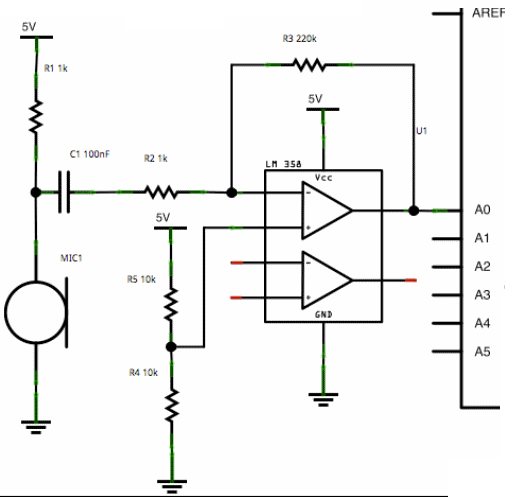
\includegraphics[width=0.8\textwidth]{high_pass_filter_circuit.png}
    \caption{High-pass filter met versterker en ADC.}
    \label{fig:circuit}
\end{figure}


\subsection{Signaalverwerking}
In figuur~\ref{fig:on_off} is zichtbaar dat het versturen van een geluidssignaal een sterk wisselend inputsignaal geeft.
\begin{figure}[ht!]
    \centering
    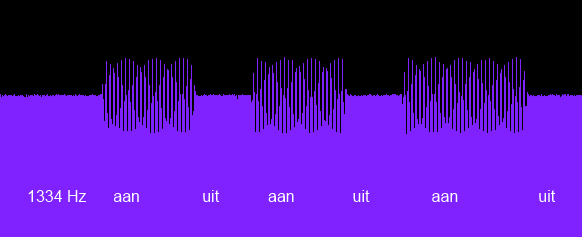
\includegraphics[width=0.8\textwidth]{resonance_on_off_commit_ff82f.png}
    \caption{Inkomend signaal bij pulserend signaal.}
    \label{fig:on_off}
\end{figure}

\begin{figure}[ht!]
    \centering
    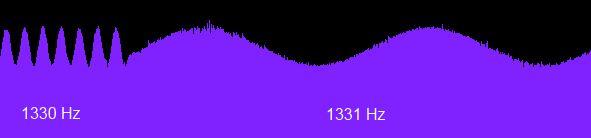
\includegraphics[width=0.8\textwidth]{resonance_2_frequencies_commit_ff82f.png}
    \caption{Inkomend signaal bij verschillende geluidsfrequencies.}
    \label{fig:resonance}
\end{figure}

% \newpage
% \appendix
% \section{Bijlage 1 - Code}
% \label{sec:code}
% % xxxxxxxxxxxxxxxxxxxxxxxxx Code Snippet STARTS xxxxxxxxxxxxxxxxxxxxxx
\lstset{
  language=C,                     % choose the language of the code
  stepnumber=1,                   % the step between two line-numbers. If it's 1, each line will be numbered
  basicstyle=\footnotesize,
 % numbersep=5pt,                 % how far the line-numbers are from the code
%  backgroundcolor=\color{white}, % choose the background color. You must add \usepackage{color}
  showspaces=false,               % show spaces adding particular underscores
  showstringspaces=false,         % underline spaces within strings
  showtabs=false,                 % show tabs within strings adding particular underscores
  tabsize=4,                      % sets default tabsize to 2 spaces
  captionpos=t,                   % sets the caption-position to top
  breaklines=true,                % sets automatic line breaking
  breakatwhitespace=true,         % sets if automatic breaks should only happen at whitespace
 % title=\lstname,                % show the filename of files included with \lstinputlisting;
 % identifierstyle=\color{identifierColor},
 % caption={Array of Pointers to Strings},
 % frame=lrtb,
 % keywordstyle=\color{purple},         % keyword style
 % commentstyle=\color{blue},           % comment style
 % stringstyle=\color{violet},          % string literal style
 belowcaptionskip = 0.2in,            % Space below caption
 abovecaptionskip = 0.2in             % Space above caption
}
% \lstset{language=C}
\begin{lstlisting}
/*
    Positioning system for Arduino One with RF24 radio chip
*/
#include <SPI.h>
#include "nRF24L01.h"
#include "RF24.h"
#include "printf.h"
#include "MatrixMath.h"

#define N (3)
// Kunstmatige waarde voor Z coordinaten
#define Z 1.0
// Percentage verschil (0 < MAX_DIFF <= 1) dat tussen twee metingen mag zitten.
#define MAX_DIFF (0.25)
// Percentage dat de nieuwste meting in het gemiddelde meetelt (0 < WEIGHT <= 1)
// Bij WEIGHT=1 wordt er geen gemiddelde bijgehouden, maar is de nieuwste meting de enige die meetelt.
#define WEIGHT (0.2)

RF24 radio(3, 9);
unsigned long radiotime;
unsigned long audiotime;
unsigned long timelimit = 50000LL;
uint8_t activeBeacon;

float pos[4][2] = { // Positions van de beacons; pos[1][1] is de y positie van beacon 1
    {0.0, 75.0},
    {72.0, 0.0},
    {294.0, 0.0},
    {372.0, 136.0}
};

float D[4];


void setup() {
  // initialize the serial communication:
  Serial.begin(9600);
  printf_begin();

  // Setup and configure rf radio
  radio.begin();
  radio.setRetries(0,0);

  radio.setDataRate(RF24_2MBPS);
  radio.setChannel(76);
  radio.setPayloadSize(1);
  radio.openReadingPipe(1, 0xdeadbeefa1LL);
  radio.openWritingPipe(0xdeadbeefa1LL);
  radio.startListening();
  radio.setAutoAck(false);
}

void loop() {
  while(radio.available()) { 
    radio.read(&activeBeacon, sizeof(uint8_t)); 
  }
  while (! radio.available());

  radiotime = micros();
  radio.read( &activeBeacon, sizeof(uint8_t));

  if(activeBeacon > 3) { return; }

  while(analogRead(A0) < 50) {
    audiotime = micros();
    if(audiotime - radiotime > timelimit) {
      return; 
    }
  }
  
  float diff = audiotime - radiotime;
  diff = diff * 0.03432; // Afstand tot beacon in cm

  //Zwak uitschieters een beetje af: max 30% increase
  if(diff > (D[activeBeacon]* (1.0 + MAX_DIFF)) && D[activeBeacon] > 0) {
    diff = D[activeBeacon] * (1.0 + MAX_DIFF);
  }
  
  if(diff < (D[activeBeacon]* (1.0 - MAX_DIFF))) {
    diff = D[activeBeacon]*(1.0 - MAX_DIFF);
  }
  
  D[activeBeacon] = D[activeBeacon]*(1.0 - WEIGHT) + diff*WEIGHT; // Weer schuivend gemiddelde */
  //D[activeBeacon] = diff;

  if(activeBeacon == 3) {
    calcPosition();
  }
}

float A[N][N];
float B[N];

void calcPosition() {
    // Relatieve afstanden tussen de nodes; gebruikt node 3 nog niet!
    A[0][0] = 2*pos[1][0] - 2*pos[0][0]; A[0][1] = 2*pos[1][1] - 2*pos[0][1]; A[0][2] = Z;
    A[1][0] = 2*pos[2][0] - 2*pos[1][0]; A[1][1] = 2*pos[2][1] - 2*pos[1][1]; A[1][2] = Z;
    A[2][0] = 2*pos[0][0] - 2*pos[2][0]; A[2][1] = 2*pos[0][1] - 2*pos[2][1]; A[2][2] = Z;
    Matrix.Invert((float*)A,N);

    B[0] = (D[0]*D[0]) - (D[1]*D[1]) - (pos[0][0]*pos[0][0]) + (pos[1][0]*pos[1][0]) - (pos[0][1]*pos[0][1]) + (pos[1][1]*pos[1][1]);
    B[1] = (D[1]*D[1]) - (D[2]*D[2]) - (pos[1][0]*pos[1][0]) + (pos[2][0]*pos[2][0]) - (pos[1][1]*pos[1][1]) + (pos[2][1]*pos[2][1]);
    B[2] = (D[2]*D[2]) - (D[0]*D[0]) - (pos[2][0]*pos[2][0]) + (pos[0][0]*pos[0][0]) - (pos[2][1]*pos[2][1]) + (pos[0][1]*pos[0][1]);
    
    float P3[N];
    Matrix.Multiply((float*)A,(float*)B,N,N,1,(float*)P3);
    printf("Position (P3): (%d,%d)\n", (int) P3[0], (int) P3[1]);
    

    // Relatieve afstanden tussen de nodes; gebruikt node 2 nog niet!
    A[0][0] = 2*pos[1][0] - 2*pos[0][0]; A[0][1] = 2*pos[1][1] - 2*pos[0][1]; A[0][2] = Z;
    A[1][0] = 2*pos[3][0] - 2*pos[1][0]; A[1][1] = 2*pos[3][1] - 2*pos[1][1]; A[1][2] = Z;
    A[2][0] = 2*pos[0][0] - 2*pos[3][0]; A[2][1] = 2*pos[0][1] - 2*pos[3][1]; A[2][2] = Z;
    Matrix.Invert((float*)A,N);

    B[0] = (D[0]*D[0]) - (D[1]*D[1]) - (pos[0][0]*pos[0][0]) + (pos[1][0]*pos[1][0]) - (pos[0][1]*pos[0][1]) + (pos[1][1]*pos[1][1]);
    B[1] = (D[1]*D[1]) - (D[3]*D[3]) - (pos[1][0]*pos[1][0]) + (pos[3][0]*pos[3][0]) - (pos[1][1]*pos[1][1]) + (pos[3][1]*pos[3][1]);
    B[2] = (D[3]*D[3]) - (D[0]*D[0]) - (pos[3][0]*pos[3][0]) + (pos[0][0]*pos[0][0]) - (pos[3][1]*pos[3][1]) + (pos[0][1]*pos[0][1]);
    float P2[N];
    Matrix.Multiply((float*)A,(float*)B,N,N,1,(float*)P2);
    printf("Position (P2): (%d,%d)\n", (int) P2[0], (int) P2[1]);
    
    
    // Relatieve afstanden tussen de nodes; gebruikt node 1 nog niet!
    A[0][0] = 2*pos[2][0] - 2*pos[0][0]; A[0][1] = 2*pos[2][1] - 2*pos[0][1]; A[0][2] = Z;
    A[1][0] = 2*pos[3][0] - 2*pos[2][0]; A[1][1] = 2*pos[3][1] - 2*pos[2][1]; A[1][2] = Z;
    A[2][0] = 2*pos[0][0] - 2*pos[3][0]; A[2][1] = 2*pos[0][1] - 2*pos[3][1]; A[2][2] = Z;
    Matrix.Invert((float*)A,N);
   
    B[0] = (D[0]*D[0]) - (D[2]*D[2]) - (pos[0][0]*pos[0][0]) + (pos[2][0]*pos[2][0]) - (pos[0][1]*pos[0][1]) + (pos[2][1]*pos[2][1]);
    B[1] = (D[2]*D[2]) - (D[3]*D[3]) - (pos[2][0]*pos[2][0]) + (pos[3][0]*pos[3][0]) - (pos[2][1]*pos[2][1]) + (pos[3][1]*pos[3][1]);
    B[2] = (D[3]*D[3]) - (D[0]*D[0]) - (pos[3][0]*pos[3][0]) + (pos[0][0]*pos[0][0]) - (pos[3][1]*pos[3][1]) + (pos[0][1]*pos[0][1]);
    float P1[N];
    Matrix.Multiply((float*)A,(float*)B,N,N,1,(float*)P1);
    printf("Position (P1): (%d,%d)\n", (int) P1[0], (int) P1[1]);
    
    
    // Relatieve afstanden tussen de nodes; gebruikt node 0 nog niet!
    A[0][0] = 2*pos[2][0] - 2*pos[1][0]; A[0][1] = 2*pos[2][1] - 2*pos[1][1]; A[0][2] = Z;
    A[1][0] = 2*pos[3][0] - 2*pos[2][0]; A[1][1] = 2*pos[3][1] - 2*pos[2][1]; A[1][2] = Z;
    A[2][0] = 2*pos[1][0] - 2*pos[3][0]; A[2][1] = 2*pos[1][1] - 2*pos[3][1]; A[2][2] = Z;
    Matrix.Invert((float*)A,N);
   
    B[0] = (D[1]*D[1]) - (D[2]*D[2]) - (pos[1][0]*pos[1][0]) + (pos[2][0]*pos[2][0]) - (pos[1][1]*pos[1][1]) + (pos[2][1]*pos[2][1]);
    B[1] = (D[2]*D[2]) - (D[3]*D[3]) - (pos[2][0]*pos[2][0]) + (pos[3][0]*pos[3][0]) - (pos[2][1]*pos[2][1]) + (pos[3][1]*pos[3][1]);
    B[2] = (D[3]*D[3]) - (D[1]*D[1]) - (pos[3][0]*pos[3][0]) + (pos[1][0]*pos[1][0]) - (pos[3][1]*pos[3][1]) + (pos[1][1]*pos[1][1]);
    float P0[N];
    Matrix.Multiply((float*)A,(float*)B,N,N,1,(float*)P0);
    printf("Position (P0): (%d,%d)\n", (int) P0[0], (int) P0[1]);
    
    // Bereken het gemiddelde van de verschillende metingen:
    int avg[N];
    avg[0] = (int) (P0[0] + P1[0] + P2[0] + P3[0]) / 4.0;
    avg[1] = (int) (P0[1] + P1[1] + P2[1] + P3[1]) / 4.0;
    avg[2] = (int) (P0[2] + P1[2] + P2[2] + P3[2]) / 4.0;
  
    printf("Position: (%d,%d)\n\n", avg[0], avg[1]);
}
\end{lstlisting}

\bibliographystyle{plain}
\bibliography{verslag_week_4}

\end{document}
